% Chapter 1
\section*{Preface}
In this chapter, we talk about the techniques used in our work to establish mechanism of a working battery. 
\pagebreak
\chapter{Techniques for characterisation} % Main chapter title
\label{chap2} % For referencing the chapter elsewhere, use \ref{Chapter1} 

\section{X-ray diffraction Studies}
X-ray diffraction is the elastic scattering of x-ray photons by atoms in a periodic lattice. Figure \ref{Figures/chap2fig:XRD} illustrates how diffraction of x-rays by crystal planes allows us to derive lattice spacings by using the Bragg's law. 

\begin{figure}[h!]
\centering
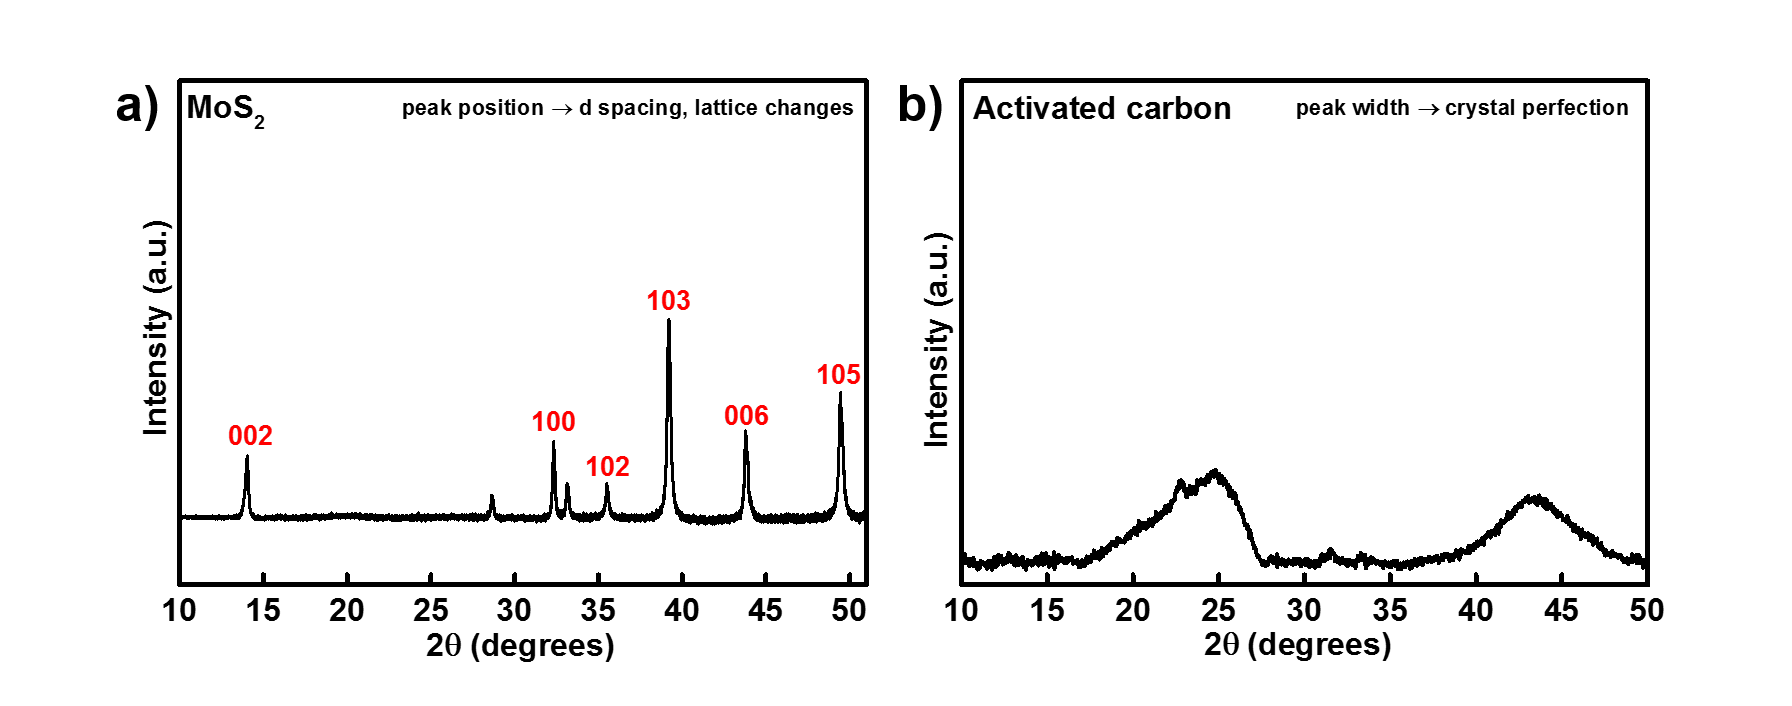
\includegraphics[width=\textwidth]{Figures/chap2fig/XRD}
\caption{a) Schematic diagram of X-ray diffraction using Bragg's law. b) XRD peak diffractogram indicating the significance of peak width and peak positions.}
\label{Figures/chap2fig:XRD}
\end{figure}
 \begin{equation} \label{eq1}
     2d\sin\theta \text= n{\lambda}
 \end{equation}
 where d = spacing between diffracting planes,\\
$\theta$ = incident angle,\\ 
n = any integer, and \\
$\lambda$ = wavelength of the incident beam. X-rays produce the diffraction pattern because their wavelength $\lambda$ is typically the same order of magnitude (1-100 $\AA$ ) as the d-spacing between the crystal planes. According to Eq.\ref{eq1} any decrease in 2$\theta$ suggests an increase in the d-spacing. 

\section{Raman spectroscopy}
Raman spectroscopy is a technique used to determine vibrational modes of molecules. It is commonly used to provide a structural fingerprint to identify molecules.

\begin{figure}[tbh!]
\centering
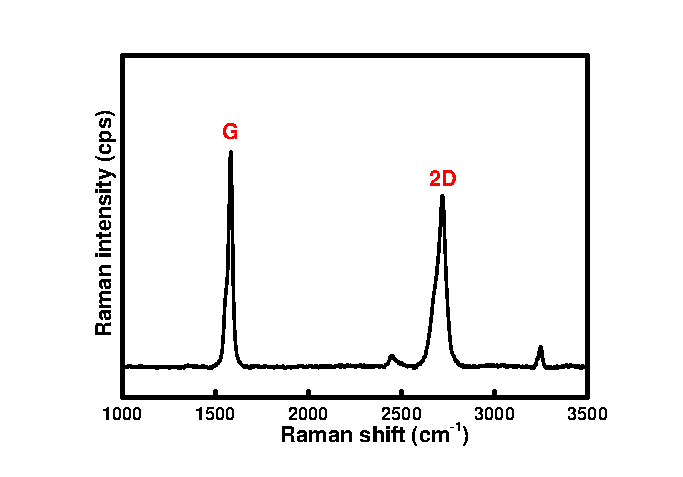
\includegraphics[width=0.5\textwidth]{Figures/chap2fig/Raman}
\caption{The sample is illuminated with a laser beam (blue box). Electromagnetic radiation from the illuminated spot is collected with a lens and sent through a Michelson interferometer (orange box), which produces interference between two beams of light. Elastic scattered radiation at the wavelength corresponding to the laser line is filtered out by a dielectric filter (blocking unwanted wavelengths), while the rest of the collected light is dispersed onto a charged coupled device (CCD)detector, which is a highly sensitive photon detector (green box).}
\label{Figures/chap2fig:Raman}
\end{figure}

This technique uses the inelastic scattering of photons, also known as Raman scattering. A source of monochromatic light, usually from a laser in the visible, near infrared, or near ultraviolet range is used (Figure \ref{Figures/chap2fig:Raman}). The laser light interacts with molecular vibrations in the system, resulting in the energy of the laser photons being shifted up (blue shift) or down (red shift). The shift in energy gives information about any changes taking place in the vibrational modes of a material. 

\section{X-ray photoelectron spectroscopy}

To measure elemental composition and oxidation states of various elements, X-ray photoelectron spectroscopy is used. It is a surface-based technique that quantitatively analyses a sample. By irradiating a sample with a beam of X-rays, kinetic energy and number of electrons escaping from the top 10 nm of the sample are measured, in Figure \ref{Figures/chap2fig:XPS}. The instrument requires high vacuum (10$^{-8}$ millibar) conditions to count these electrons. The electron emission after irradiation is also called a 'photoelectron effect'. These electrons are separated according to their energies and counted. A normal XPS spectrum is a plot of the number of electrons detected versus the binding energy of the electrons detected. The set of XPS peaks produced at certain binding energies values helps in identifying all the elements, and their chemical environment, that exist in the sample. 

\begin{figure}[tbh!]
\centering
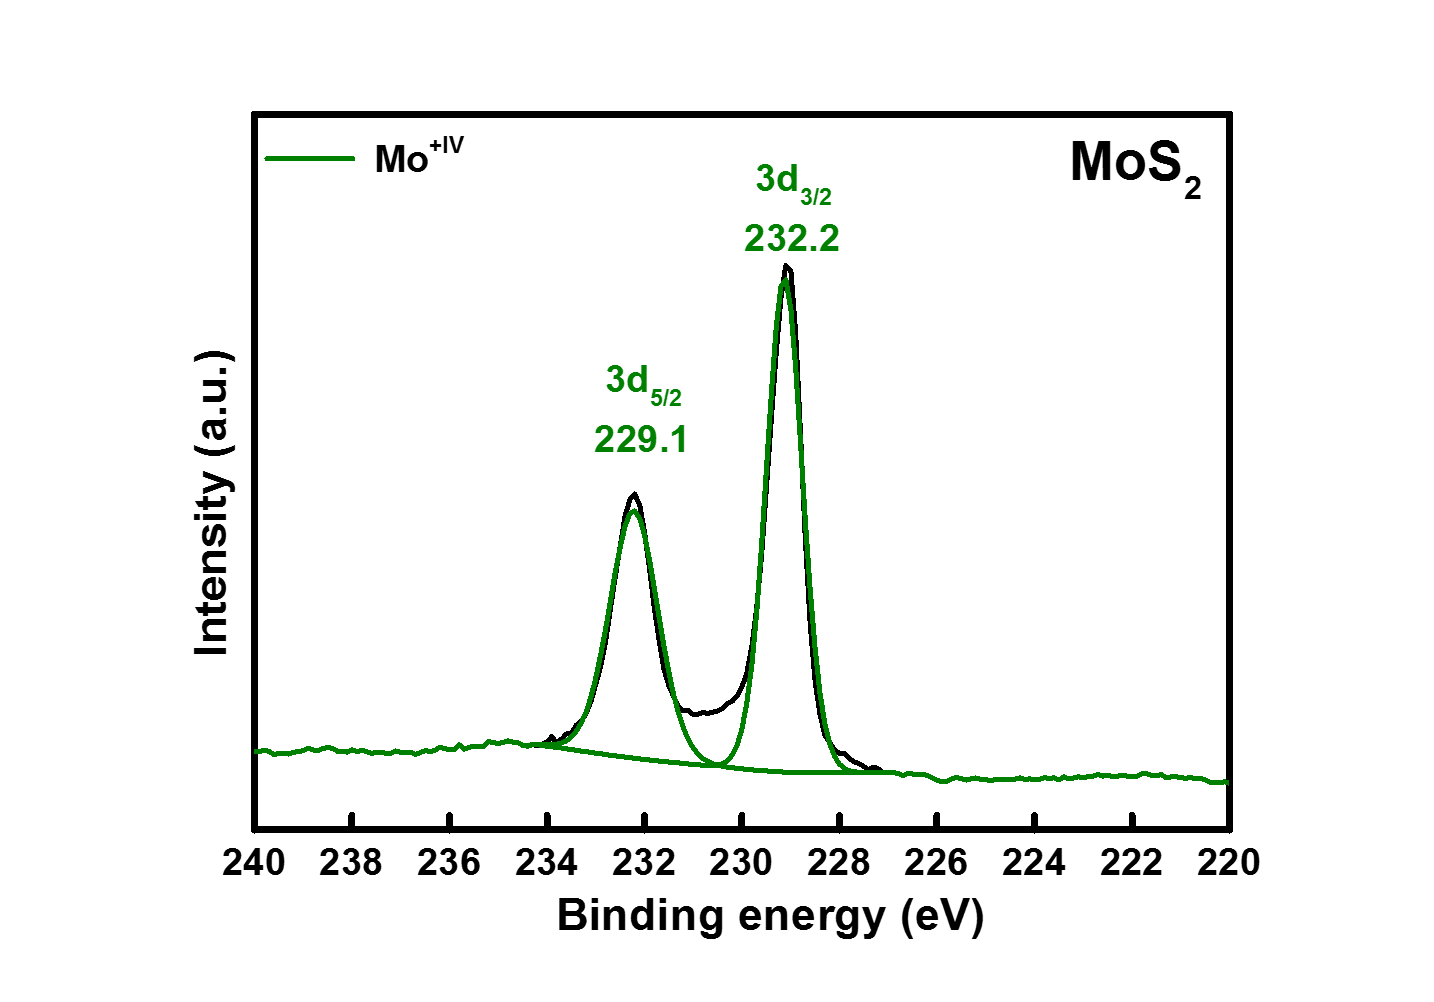
\includegraphics[width=0.5\textwidth]{Figures/chap2fig/XPS}
\caption{Schematic for a X-ray photoelectron spectrometer.}
\label{Figures/chap2fig:XPS}
\end{figure}

In practice, XPS detects all elements from lithium and above. It cannot easily detect hydrogen or helium because helium has a very small cross-sectional area for photoemission and hydrogen only has one electron which is used in making bonds with  small photoelectron cross-section. Detection limits for most of the elements are in the parts per thousand range. XPS is used to study redox processes taking place in a cell. For example, in Al/\ce{MoSe2} cells, molybdenum oxidised from \ce{Mo^{+4}} to \ce{Mo^{5+}} when the cells charged. 

\section{Cyclic voltammetry}
Cyclic voltammetry (CV) is a technique which measures the current that develops in an electrochemical cell during oxidation and reduction of an analyte (say M). It is performed by cycling the potential of a working electrode, and measuring the resulting current. In Figure \ref{Figures/chap2fig:CV}, we started a forward sweep with a positive scan (lower potential to higher potential). S1 is called a switch potential where the voltage is sufficient enough to cause an oxidation or reduction, and the scan is reversed. Potential is then swept negatively (higher potential to lower potential) until it reaches S2 (another switch potential). In an ideal situation, during forward sweep, M is depleted from the solution as it gets oxidised to \ce{M+}. Further oxidation after scanning higher potentials, leads to growth of a diffusion layer (solution containing M/\ce{M+} ions) at the electrode surface throughout the scan. The layer continues to expand until a certain point, recording maximum current density. However, since diffusion layer continues to grow at this stage, flux of M from the bulk solution to electrode surface decreases. Therefore, current starts to decrease and we get an oxidation peak. A reverse scan converts \ce{M+} back to M (reduction) via similar pathway- formation of a diffusion layer containing M and eventually we record a reduction peak. The two peaks are separated due to the diffusion of the analyte to and from the electrode. If the reduction process is chemically and electrochemically reversible, a peak-to-peak separation of 57 mV is observed \cite{bard_electrochemical_1980}. When there is a high barrier to electrochemical irreversibility, electron transfer reactions are sluggish and more positive/negative potentials are required to observe oxidation/reduction reactions respectively. 

\begin{figure}[tbh!]
\centering
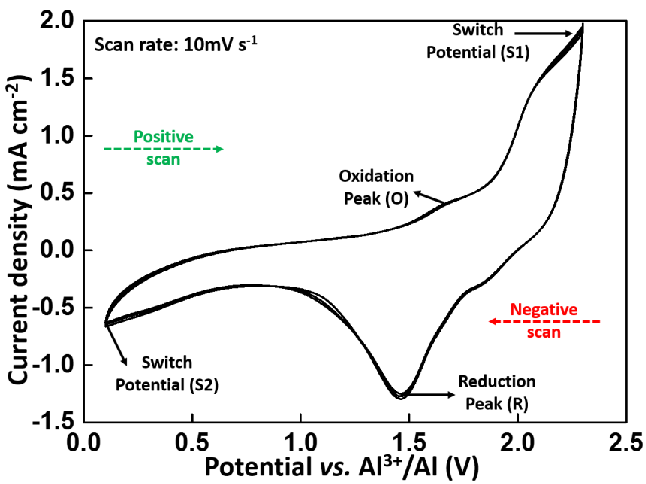
\includegraphics[width=0.8\textwidth]{Figures/chap2fig/CV}
\caption{Cyclic voltammogram of an AIB at a scan rate of 10 mV s$^{-1}$ using a two-electrode cell with aluminium foil acting as a counter and reference electrode.}
\label{Figures/chap2fig:CV}
\end{figure}

Scan rates play a very important role too. If a CV is run on a slower scan rate (0.05 mV s$^{-1}$), diffusion layer grows farther from the electrode, which reduces the flux, consequently decreasing the current value. At a faster scan rate lead (1 V s$^{-1}$), the size of the diffusion layer decreases and higher currents are recorded. Cyclic voltammetry is a helpful tool in understanding the presence of a surface reaction and its reversibility during cell cycles. It can be used for both single-electron and multi-electron processes.  

\section{Galvanostatic charge/discharge cycles}
Galvanostatic  charge and discharge is a method to evaluate the amount of charge stored in a cell typically under constant current. The technique measures voltage at a controlled or fixed current rate. Since the current is repeatedly reversed, it is also known as 'cyclic chronopotentiometry'. It is generally used to estimate their specific capacities and cycling stability of a cell. The total quantity of electricity per mass available from a fully charged cell can be calculated, from the charge transferred during discharge in terms of mAh g$^{-1}$. Specific discharge capacity is frequently measured at different discharging rates to establish rate capability of a cell \cite{pyun_electrochemistry_2012-1}. The voltage profile obtained can be used to identify multi-step redox reactions, in Figure \ref{Figures/chap2fig:ChrononCDC}. 

\begin{figure}[tbh!]
\centering
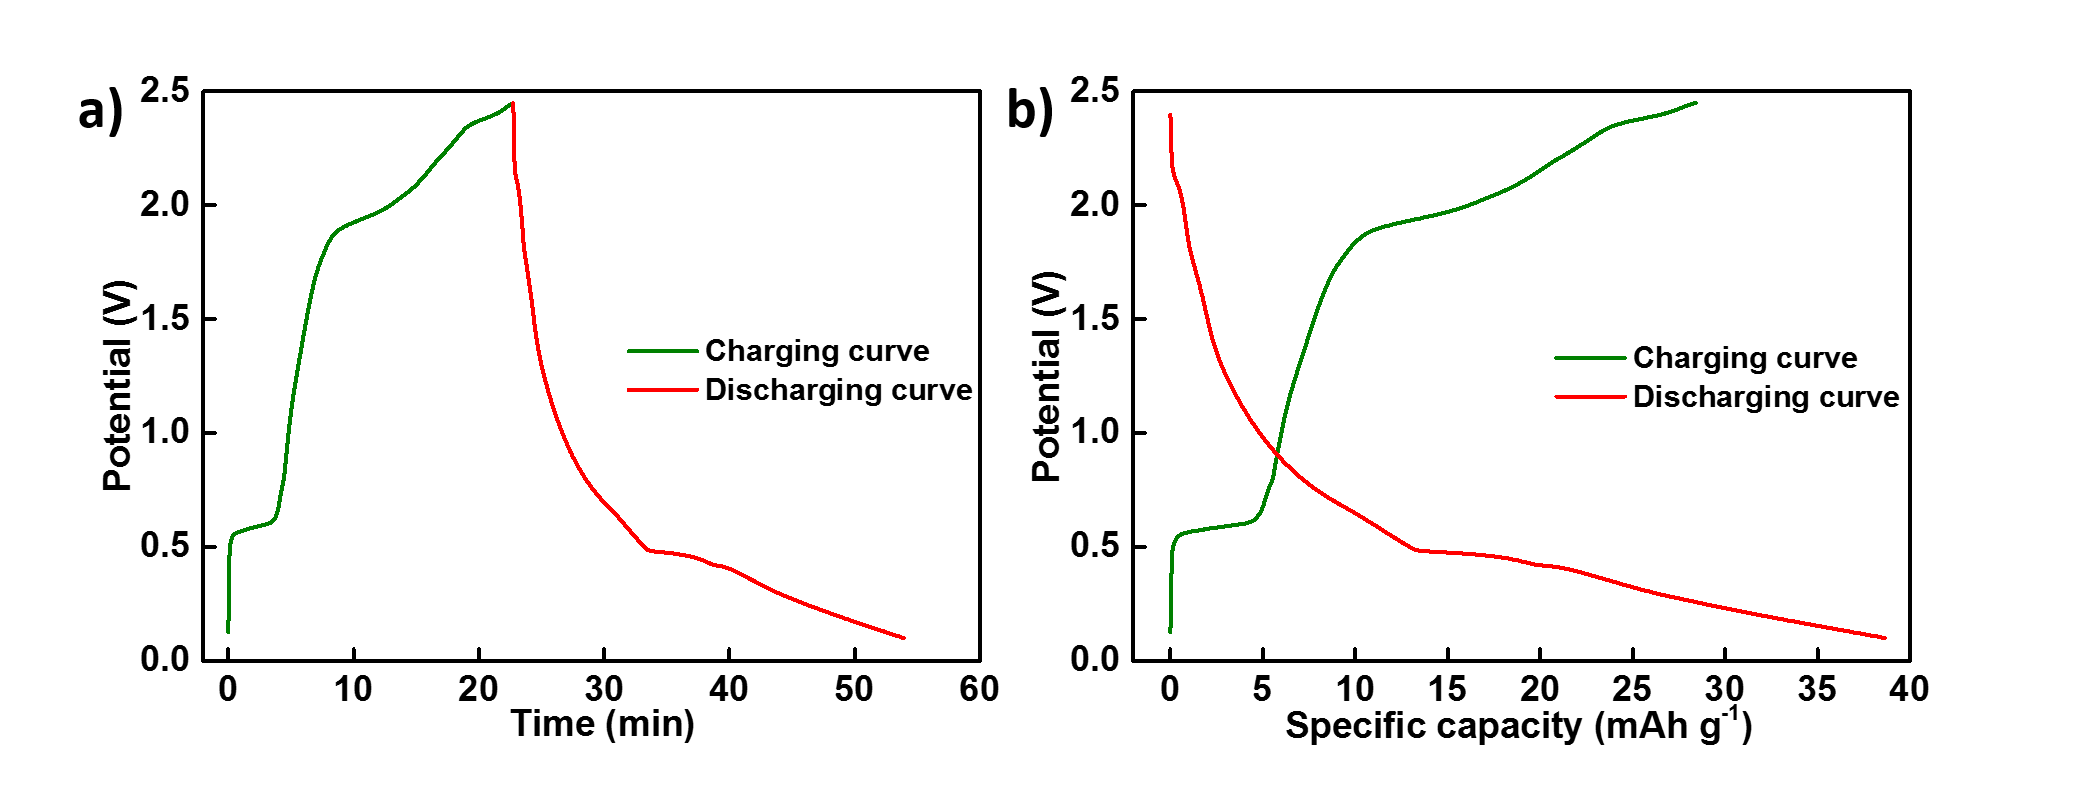
\includegraphics[width=\textwidth]{Figures/chap2fig/ChrononCDC}
\caption{a) Chronopotentiogram- a graph of electric potential versus time, at constant current. b) A galvanostatic charge/discharge curve showing the voltage plateaus at which reactions occur and the charging/discharging capacity.}
\label{Figures/chap2fig:ChrononCDC}
\end{figure}
